% -----------------------------------
% -----------------------------------
% abnTeX2: Normas ABNT NBR 14724:2011 + sugestões FGV/EMAp. 

% Autor: Lauro César Araujo
% Adaptações EMAp: Lucas Machado Moschen 
% Copyright 2012-2018 by abnTeX2 group at http://www.abntex.net.br/ 

%% This work may be distributed and/or modified under the
%% conditions of the LaTeX Project Public License, either version 1.3
%% of this license or (at your option) any later version.
%% The latest version of this license is in
%%   http://www.latex-project.org/lppl.txt
%% and version 1.3 or later is part of all distributions of LaTeX
%% version 2005/12/01 or later.
% ----------------------------------
% ----------------------------------
\documentclass[
	% -- opções da classe memoir --
	12pt,				% tamanho da fonte
	%openright,			% capítulos começam em página ímpar (insere página vazia caso preciso)
	oneside,			% para impressão em recto e verso. Oposto a oneside
	a4paper,			% tamanho do papel. 
	% -- opções da classe abntex2 --
	%chapter=TITLE,		% títulos de capítulos convertidos em letras maiúsculas
	%section=TITLE,		% títulos de seções convertidos em letras maiúsculas
	%subsection=TITLE,	% títulos de subseções convertidos em letras maiúsculas
	%subsubsection=TITLE,% títulos de subsubseções convertidos em letras maiúsculas
	% -- opções do pacote babel --
	english,			% idioma para inglês
	brazil				% idioma para português
	]{abntex2}

%------------------------------------------------
%-------------- Pacotes necessários -------------
%------------------------------------------------

% Escrita 
\usepackage[T1]{fontenc}
\usepackage[utf8]{inputenc}
\usepackage{lmodern}
\usepackage{microtype} % para melhorias de justificação
\usepackage{indentfirst}

\renewcommand{\ABNTEXchapterfont}{\fontfamily{ptm}\fontseries{b}\selectfont}

% Gráficos 
\usepackage{color}
\usepackage{caption}
\usepackage{subcaption}
\usepackage{graphicx}
\graphicspath{{../../images/}}

% Matemáticos 
\usepackage{amsthm, amssymb, amsmath, mathtools}

% Outros 
\usepackage{tabularx}
\usepackage{listings}
\renewcommand{\lstlistingname}{Código}
\renewcommand{\lstlistlistingname}{Lista de códigos}
\lstset{basicstyle=\ttfamily\footnotesize,breaklines=true, numbers=left,
inputencoding=utf8, extendedchars=true, frame=single,
literate=%
        {é}{{\'{e}}}1
        {è}{{\`{e}}}1
        {ê}{{\^{e}}}1
        {ë}{{\¨{e}}}1
        {É}{{\'{E}}}1
        {Ê}{{\^{E}}}1
        {û}{{\^{u}}}1
        {ù}{{\`{u}}}1
        {ú}{{\'{u}}}1
        {â}{{\^{a}}}1
        {à}{{\`{a}}}1
        {á}{{\'{a}}}1
        {ã}{{\~{a}}}1
        {Á}{{\'{A}}}1
        {Â}{{\^{A}}}1
        {Ã}{{\~{A}}}1
        {ç}{{\c{c}}}1
        {Ç}{{\c{C}}}1
        {õ}{{\~{o}}}1
        {ó}{{\'{o}}}1
        {ô}{{\^{o}}}1
        {Õ}{{\~{O}}}1
        {Ó}{{\'{O}}}1
        {Ô}{{\^{O}}}1
        {î}{{\^{i}}}1
        {Î}{{\^{I}}}1
        {í}{{\'{i}}}1
        {Í}{{\~{Í}}}1
}

% Citações 
%\usepackage[brazilian,hyperpageref]{backref}
%\usepackage[alf]{abntex2cite}	% Citações padrão ABNT
\usepackage[style=abnt]{biblatex}
\addbibresource{biblio.bib}  

% \renewcommand{\backrefpagesname}{Citado na(s) página(s):~}
% % Texto padrão antes do número das páginas
% \renewcommand{\backref}{}
% % Define os textos da citação
% \renewcommand*{\backrefalt}[4]{
% 	\ifcase #1 %
% 		Nenhuma citação no texto.%
% 	\or
% 		Citado na página #2.%
% 	\else
% 		Citado #1 vezes nas páginas #2.%
% 	\fi}%
% ---

%----------------------------------------
%------- Capa e Folha de Rosto ----------
%----------------------------------------

\newcommand\subtitulo[1]{\def\@subtitulo{#1}}
\newcommand{\imprimirsubtitulo}{\@subtitulo}

\renewcommand{\imprimircapa}{%
	\begin{capa}%
	\center
		\ABNTEXchapterfont\Large \MakeUppercase{\imprimirinstituicao}
		\\\vspace*{4cm}
		{\ABNTEXchapterfont\large \MakeUppercase{\imprimirautor}}
		\vfill
		\begin{center}
		\ABNTEXchapterfont\large\MakeUppercase{\imprimirtitulo}\normalfont\MakeUppercase{:
		\imprimirsubtitulo}
		\end{center}
		\vfill
		\normalfont\large\imprimirlocal
		\\\normalfont\large\imprimirdata
		\vspace*{1cm}
	\end{capa}
}

\makeatletter
\renewcommand{\folhaderostocontent}{
  \begin{center}

    %\vspace*{1cm}
    {\ABNTEXchapterfont\large\MakeUppercase{\imprimirautor}}
	
    \vspace*{\fill}\vspace*{\fill}
    \begin{center}
      \ABNTEXchapterfont\bfseries\large\MakeUppercase{\imprimirtitulo}\normalfont\MakeUppercase{:
      \imprimirsubtitulo}
    \end{center}
    \vspace*{\fill}
	
    \abntex@ifnotempty{\imprimirpreambulo}{%
      \hspace{7.5cm}
      \begin{minipage}{.5\textwidth}
      	\SingleSpacing
         \imprimirpreambulo
         \\\\
         Orientador: \imprimirorientador
       \end{minipage}%
       \vspace*{\fill}
    }%

    % {\large\imprimirorientadorRotulo~\imprimirorientador\par}
    % \abntex@ifnotempty{\imprimircoorientador}{%
    %    {\large\imprimircoorientadorRotulo~\imprimircoorientador}%
    % }%
    \vspace*{\fill}

    {\large\imprimirlocal}
    \par
    {\large\imprimirdata}
    \vspace*{1cm}

  \end{center}
}
\makeatother

\titulo{Geodesic Tracing}
\subtitulo{Visualização de curvas e superfícies através de geodésicas}
\autor{Cristhian Grundmann}
\orientador{Asla Medeiros e Sá}
\local{Rio de Janeiro}
\data{2022}
\instituicao{%
  Fundação Getulio Vargas \\
  \par
  Escola de Matemática Aplicada
}
\tipotrabalho{Trabalho de Conclusão de Curso}

\preambulo{Trabalho de conclusão de curso apresentada para a Escola de
Matemática Aplicada (FGV/EMAp) como requisito para o grau de bacharel em
Matemática Aplicada. \\ \\ Área de estudo: curvas e superfícies.}


%---------------------------------------------
%-------------------- PDF --------------------
%---------------------------------------------

% alterando o aspecto da cor azul
\definecolor{blue}{RGB}{41,5,195}

% informações do PDF
\makeatletter
\hypersetup{
     	%pagebackref=true,
		pdftitle={\@title}, 
		pdfauthor={\@author},
    	pdfsubject={\imprimirpreambulo},
	    pdfcreator={LaTeX with abnTeX2},
		pdfkeywords={abnt}{latex}{abntex}{abntex2}{trabalho acadêmico}, 
		colorlinks=true,       		% false: boxed links; true: colored links
    	linkcolor=blue,          	% color of internal links
    	citecolor=blue,        		% color of links to bibliography
    	filecolor=magenta,      		% color of file links
		urlcolor=blue,
		bookmarksdepth=4
}
\makeatother

% Posiciona figuras e tabelas no topo da página quando adicionadas sozinhas
% em um página em branco. Ver https://github.com/abntex/abntex2/issues/170
\makeatletter
\setlength{\@fptop}{5pt} % Set distance from top of page to first float
\makeatother

%---------------------------------------
%--------- Mais configurações-----------
%---------------------------------------

% Possibilita criação de Quadros e Lista de quadros.
% Ver https://github.com/abntex/abntex2/issues/176
\newcommand{\quadroname}{Quadro}
\newcommand{\listofquadrosname}{Lista de quadros}

\newfloat[chapter]{quadro}{loq}{\quadroname}
\newlistof{listofquadros}{loq}{\listofquadrosname}
\newlistentry{quadro}{loq}{0}

% configurações para atender às regras da ABNT
\setfloatadjustment{quadro}{\centering}
\counterwithout{quadro}{chapter}
\renewcommand{\cftquadroname}{\quadroname\space} 
\renewcommand*{\cftquadroaftersnum}{\hfill--\hfill}

\setfloatlocations{quadro}{hbtp} % Ver https://github.com/abntex/abntex2/issues/176

%-----------------------------------------------------
%--------------------- Margens -----------------------
%-----------------------------------------------------

\setlrmarginsandblock{3cm}{2cm}{*}
\setulmarginsandblock{3cm}{2cm}{*}
\checkandfixthelayout

%-----------------------------------------------------
%------ Espaçamentos entre linhas e parágrafos -------
%-----------------------------------------------------

% O tamanho do parágrafo é dado por:
\setlength{\parindent}{1.3cm}

% Controle do espaçamento entre um parágrafo e outro:
\setlength{\parskip}{0.2cm}  % tente também \onelineskip

% compila o índice
\makeindex

%------------------------------------------------------
%----------- Personal Definitions ---------------------
%------------------------------------------------------

\newcommand{\R}{\mathbb{R}}
\newcommand{\x}{\boldsymbol{x}}
\newcommand{\N}{\operatorname{Normal}}
\newcommand{\betadist}{\operatorname{Beta}}
\newcommand{\bern}{\operatorname{Bernoulli}}
\newcommand{\tril}{\operatorname{tril}}

\newcommand{\ev}{\mathbb{E}}
\newcommand{\var}{\operatorname{Var}}
\newcommand{\cor}{\operatorname{Cor}}
\newcommand{\cov}{\operatorname{Cov}}

\newtheorem{theorem}{Theorem}[]
\newtheorem{proposition}{Proposition}[]

\theoremstyle{definition}
\newtheorem{definition}{Definition}[section]

\theoremstyle{remark}
\newtheorem*{remark}{Remark}
\newtheorem{assumption}{Assumption}

\newcommand{\improve}[1]{\textcolor{red}{#1}}

%-------------------------------------------------
%----------------- Document ----------------------
%-------------------------------------------------

\begin{document}

\newcounter{num}
% if num != 1, do not print the pre textual 
\setcounter{num}{1}

\selectlanguage{brazil}
\frenchspacing 

%----------------------------------------------
%--------------- Pré-textuais -----------------
%----------------------------------------------
%\pretextual

\imprimircapa

\ifnum\value{num}=1
{\imprimirfolhaderosto*

%\begin{fichacatalografica}
	\sffamily
	\vspace*{\fill}					% Posição vertical
	\begin{center}					
	\fbox{\begin{minipage}[c][8cm]{13.5cm}		% Largura
	\small
	Ficha catalográfica elaborada pela BMHS/FGV \\

	%\imprimirautor
	Moschen, Lucas Machado % Paginas com as citações na bibl
	
	\hspace{0.5cm} \imprimirtitulo / \imprimirautor. -- \imprimirdata.
	
	\hspace{0.5cm} \thelastpage f.\\
		
	\hspace{0.5cm}
	\parbox[t]{\textwidth}{\imprimirtipotrabalho~--~School of Applied
	Mathematics.}\\
	
	\hspace{0.5cm} Advisor: \imprimirorientador .

	\hspace{0.5cm} Includes bibliography. \\
	
	\hspace{0.5cm}
		1. Bayesian statistics.
		2. Respondent-driven Sampling.
		2. Sensitivity and specificity.
		I. Carvalho, Luiz Max.
		II. School of Applied Mathematics.
		III. \imprimirtitulo 			
	\end{minipage}}
	\end{center}
\end{fichacatalografica}

% Uncomment if you have the pdf 
% \begin{fichacatalografica}
%     \includepdf{fig_ficha_catalografica.pdf}
% \end{fichacatalografica}

%\begin{errata}

\begin{table}[htb]
    \center
    \footnotesize
    \begin{tabular}{|p{1.4cm}|p{1cm}|p{3cm}|p{3cm}|}
    \hline
    \textbf{Folha} & \textbf{Linha} & \textbf{Onde se lê} &
    \textbf{Leia-se}\\
    \hline
    17 & 8 & Matemtica & Matemática \\
    \hline
    \end{tabular}
\end{table}

\end{errata}

%\begin{folhadeaprovacao}

    \begin{center}
      {\ABNTEXchapterfont\large\MakeUppercase{\imprimirautor}}
  
      \vspace*{\fill}\vspace*{\fill}
      \begin{center}
        \ABNTEXchapterfont\bfseries\large\MakeUppercase{\imprimirtitulo}\normalfont\MakeUppercase{:
        \imprimirsubtitulo}	
      \end{center}
      \vspace*{\fill}
      
      \hfill
      \begin{minipage}{.7\textwidth}
          \imprimirpreambulo \\ \\
          E aprovado em ?/12/2022 \\
          Pela comissão organizadora
      \end{minipage}%
      \vspace*{\fill}
     \end{center}
  
     \assinatura{\imprimirorientador \\ Escola de Matemática Aplicada} 
     \assinatura{Convidado 1 \\ Instituição 1}
     \assinatura{Convidado 2 \\ Instituição 2}
     %\assinatura{\textbf{Professor} \\ Convidado 3}
     %\assinatura{\textbf{Professor} \\ Convidado 4}
\end{folhadeaprovacao}

% \begin{folhadeaprovacao}
% \includepdf{folhadeaprovacao_final.pdf}
% \end{folhadeaprovacao}

%\begin{dedicatoria}
    \vspace*{\fill}
    %\noindent
    \hfill
    \begin{minipage}{.6\textwidth}
     Dedico essa dissertação a todas que lutaram para que eu estivesse aqui. 
    \end{minipage}
\end{dedicatoria}
 
\begin{agradecimentos}
    Lembre de agradecer a quem te apoiou, como, por exemplo, orientador,
    família, agência de fomento, professores conselheiros. 
\end{agradecimentos}

\begin{epigrafe}
\vspace*{\fill}

\begin{flushright}
    \hspace{7.5cm}
    \textit{
        ``If your experiment needs a statistician, you need a better
        experiment.''} \\
        \textit{Ernest Rutherford}
\end{flushright}
\end{epigrafe}

%\setlength{\absparsep}{18pt} 
\begin{resumo}[Resumo]
Curvas e superfícies costumam ser visualizados em um espaço ambiente 2D ou 3D.
Esse projeto implementa essa visualização em 3D, e para superfícies,
implementa também o \textit{Geodesic Tracing}: uma visualização intrínseca à
superfície, baseada em curvas geodésicas. Além de curvas e superfícies,
o projeto permite visualizar pontos e vetores. Outros objetos auxiliares podem ser
definidos, como parâmetros(controles deslizantes), funções e grades para
instanciar objetos múltiplas vezes.

Para a especificação dos objetos, uma linguagem textual foi estabelecida,
acompanhada de um compilador capaz de transformar o texto em estruturas de dados
úteis para a renderização. A linguagem é descrita por uma gramática livre-de-contexto
inambígua.

Para a interface gráfica, \textit{OpenGL} é usado para a renderização,
e \textit{Dear ImGUI} é usado para construir os controles e janelas.

O resultado é um sistema de performance em tempo real, testado sem
inconsistências. A estética dos gráficos, da interface e da
linguagem não foram negligenciados, e se tornaram bastante agradáveis.

 Palavras-chave: visualização. curvas. superfícies. compilador.
\end{resumo}

\begin{resumo}[Abstract]
\begin{otherlanguage*}{english}
Curves and surfaces are usually visualized in a 2D or 3D ambient space.
This project implements this visualization in 3D, and for surfaces, also
implements the \textit{Geodesic Tracing}: an intrinsic visualization of the surface,
based on geodesic curves. Points and vectors can also be visualized.
Other auxiliary objects can be defined, like parameters(with slider controls),
functions and grids to instantiate objects.

A textual language was designed for the specification of these objects,
accompanied by a compiler capable of transforming the text into data structures
that are useful for rendering. This language is described by an unambiguous context-free grammar.

For the graphical interface, \textit{OpenGL} is used to do the rendering,
and \textit{Dear ImGUI} is used to build GUI components like buttons and windows.

The result is a system with real-time performance, tested without any inconsistencies.
The aesthetic of the graphics, the interface and the language weren't
overlooked, and became quite pleasing.

 Keywords: visualization. curves. surfaces. compiler.
\end{otherlanguage*}
\end{resumo}

%\pdfbookmark[0]{\listfigurename}{lof}
%\listoffigures*
%\cleardoublepage

% \pdfbookmark[0]{\listofquadrosname}{loq}
% \listofquadros*
% \cleardoublepage

%\pdfbookmark[0]{\listtablename}{lot}
%\listoftables*
%\cleardoublepage

%\begin{siglas}
    \item[CDC] Centers for Disease Control and Prevention
    \item[HIV] Human immunodeficiency virus  
  \end{siglas}
  
  \begin{simbolos}
    \item[$\in$] Belongs to 
    \item[$\Sigma_{i=1}^n x_i$] Sum of the variables $x_1, x_2, \dots, x_n$
    \item[$\Pr(A)$] Probability of an event $A$
    \item[$M^T$] Transpose of matrix $M$
    \item[$\ind$] Indicator function 
    \item[$\operatorname{tril}(M)$] Lower triangle matrix of $M$
    \item[$\R_{>0}$] Set of positive real numbers
    \item[$\det(M)$] Determinant of $M$ 
    \item[$\sim$] Is distributed as 
    \item[$iid$] Independent and identically distributed
    \item[$\Phi$] Normal cumulative distribution
    \item[$\exp$] Exponential  
    \item[$\int$] Integral 
    \item[$\ev(X)$] Expected value of random variable $X$ 
    \item[$\var(X)$] Variance of random variable $X$
    \item[$A^*$] Hermitian matrix of $A$ 
  \end{simbolos}


\pdfbookmark[0]{\listtablename}{loc}
\lstlistoflistings
\cleardoublepage

}\fi

\pdfbookmark[0]{\contentsname}{toc}
%\tableofcontents*
\cleardoublepage

% ----------------------------------------------------------
% ELEMENTOS TEXTUAIS
% ----------------------------------------------------------
\textual

\chapter{Introdução}
Desenhos de superfícies costumam ser feitos a partir de um ponto de vista do
espaço ambiente 3D ou 2D, como em MatLab, Mathematica e Geogebra.
Uma curva ou superfície é definida numa linguagem e então é renderizada.
Uma forma muito comum de renderização é a discretização da curva ou superfície,
formando segmentos no caso de uma curva, ou triângulos para superfícies.
O usuário então pode interagir com a software, podendo mudar a orientação e a posição
da câmera.

O objetivo desse projeto é a visualização de curvas e superfícies.
Esse projeto também implementa uma visualização de superfícies que não depende de um espaço ambiente.
Para isso, é necessário uma imagem sobre a superfície, para poder observá-la.

A visualização pode ser comparada ao que um ser bidimensional interno à superfície observaria:
simula-se raios de luz partindo da posição do ser, e os pontos iluminados são observados.
Os raios de luz devem seguir caminhos em `linha reta', que minimizam distância.
Para uma superfície qualquer, esses caminhos são chamados de geodésicos,
estudados na geometria diferencial, e descritos no capítulo \ref{geomdiff}.
A visualização, chamada de \textit{geodesic tracing}, renderiza a imagem sobre a superfície,
e suas curvaturas podem ser notadas. Ao se mover, a imagem observada pode se distorcer,
dependendo da curvatura.

A implementação desse projeto é feita em três partes:
compilador, método numérico e interface gráfica.

O compilador fornece uma maneira do usuário definir as superfícies e outros objetos.
O usuário escreve um texto, seguindo algumas regras gramaticais, que então é processado.
A teoria de compiladores é essencial para essa etapa,
principalmente a análise léxica e a análise sintática \cite{Dragon:1}.
O compilador está descrito no capítulo \ref{comp}.
A linguagem, com exemplos de programas, está descrita no capítulo \ref{lang}.

O método numérico se refere à simulação dos raios de luz na superfície.
Um raio de luz é determinado pela posição e direção inicial, que são as condições iniciais.
Um sistema de equações diferenciais ordinárias(equação geodésica \cite{GeomDiff:1})
determina a curva que a luz traça.
Uma solução aproximada da equação é calculada pelo método de Runge-Kutta de ordem 4 \cite{Anal:1}.
O método está descrito no capítulo \ref{numeric}.

A interface gráfica é simples e é construída usando \textit{Dear ImGUI} \cite{ImGui},
uma ferramenta de interface gráfica fácil de usar.
A linguagem de programação escolhida para a implementação desse projeto é \textit{C++},
e para desenhar a interface e os objetos, \textit{OpenGL} é usado.
A interface está descrita no capítulo \ref{interface}.

O objetivo primário desse projeto é a visualização de curvas, superfícies, e o geodesic tracing.
Porém, a estética dos gráficos e da linguagem descritiva, performance
e robustez do sistema também são levados em consideração.

% ----------------------------------------------------------
% Finaliza a parte no bookmark do PDF
% para que se inicie o bookmark na raiz
% e adiciona espaço de parte no Sumário
% ----------------------------------------------------------
\phantompart

\chapter{Linguagem}
\label{lang}

O usuário se comunica com a interface através de um texto, chamado de programa,
que contém os objetos de interesse. 
Por exemplo, em GeoGebra, o círculo unitário pode ser
definido como
\texttt{c = Curve(cos(t), sin(t), t, 0, 2pi)}.
Na linguagem desse projeto, a definição seria
\texttt{curve c(t) = (cos(t), sin(t), 0), t : [0, 2pi];}.

O código \ref{ex1} é um exemplo.
\begin{lstlisting}[caption=Exemplo de objetos,label=ex1]
#circle and tangents
param r : [/2, 1];
param o : [0, 2pi];
curve c(t) = r(cost, sint, 0), t : [0, 2pi];
grid k : [0, 2pi, 8];
define k2 = k + o;
point p = ck2;
vector v = c'k2 @ p;

#function and surface
#function f(x, y) = x^2+y^2;
#surface s(u,v) = (u,v,f(u,v)), u : [-1, 1], v : [-1, 1];
\end{lstlisting}

A linguagem permite comentários no estilo da linguagem Python, usando \texttt{\#}.

O programa declara os seguintes objetos:

\begin{centering}
\begin{tabularx}{\textwidth}{||c|X||}
    \hline
    \texttt{r} e \texttt{o} & parâmetros que podem ser alterados na interface.
    Seus valores devem estar nos intervalos indicados. \\ 

    \hline
    \texttt{c} & uma curva parametrizada por \texttt{t}.
    O domínio da parametrização é o intervalo indicado.
    A curva depende do parâmetro \texttt{r}, que foi definido anteriormente. \\

    \hline
    \texttt{k} & uma grade de 8 pontos igualmente espaçados no intervalo indicado.
    Uma grade é tratada como uma constante, assim como um parâmetro.
    Se um objeto desenhável depende de uma grade, uma instância é desenhada para cada valor da grade.
    Um objeto pode depender de mais de uma grade. \\

    \hline
    \texttt{k2} & uma constante, e não pode ser alterada na interface como os parâmetros.
    Esse tipo de objeto pode ser usado para deixar o programa mais legível. \\
    
    \hline
    \texttt{p} & o ponto da curva \texttt{c} de parâmetro \texttt{t = k2}.
    Esse objeto depende indiretamente de \texttt{k}, então é instanciado 8 vezes. \\
    
    \hline
    \texttt{v} & o vetor tangente da curva \texttt{c} no ponto \texttt{p} 
    e desenhado a partir do mesmo ponto.
    O vetor também depende indiretamente de \texttt{k}, então é desenhado 8 vezes. \\
    \hline
\end{tabularx}
\end{centering}

A figura \ref{img:ex1} demonstra os objetos declarados em perspectiva 3D.
\begin{figure}[!ht]
    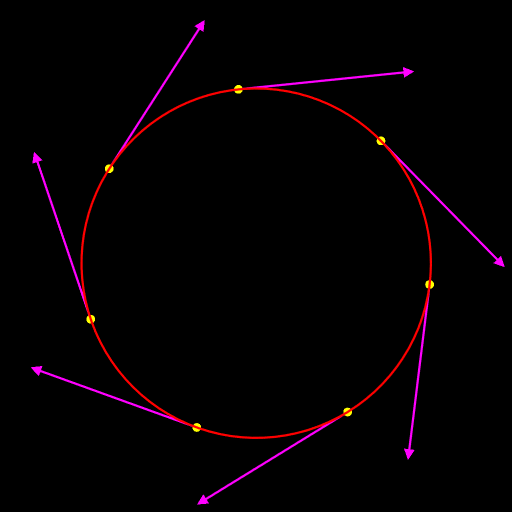
\includegraphics[width=\linewidth]{ex1.png}
    \caption{Exemplo 1}
    \label{img:ex1}
\end{figure}

Os objetos \texttt{f} e \texttt{s} estão comentados, então não são considerados.
Estão presentes apenas para o exemplo ter todos os tipos de objeto.

A linguagem de descrição de objetos não é trivial, nem sua sintaxe matemática,
que possui elementos inventados para esse projeto.
A seguir, uma breve lista de observações:

\begin{itemize}
\item
Os objetos desenháveis são pontos, vetores, curvas e superfícies.
Pontos e vetores podem ser usados em outros objetos, sendo tratados como tuplas.
Por exemplo, \texttt{v} usa o ponto \texttt{p}.
Curvas e superfícies podem ser usadas como funções, mas sem a restrição no domínio.
Por exemplo, \texttt{p} usa \texttt{c} como função.
Um objeto só pode se referir aos objetos definidos anteriormente.
Os parâmetros das curvas e superfícies podem ter qualquer nome disponível.

\item
Há duas constantes pré-definidas: \texttt{pi} e \texttt{e};
e diversas funções pré-definidas:
\texttt{sin}, \texttt{cos}, \texttt{tan},
\texttt{exp}, \texttt{log}, \texttt{sqrt} e \texttt{id}.
A função \texttt{id} é a identidade é útil apenas no funcionamento interno do sistema.

\item
Parâmetros e grades podem ser multidimensionais:
\texttt{param T : [0, 1], [0, 1];}. Assim, o objeto \texttt{T} é uma tupla,
e seus elementos podem ser obtidos com \texttt{T\_1} e \texttt{T\_2}.

\item As grades das curvas e superfícies são por padrão 100 e 100x100, respectivamente.
É possível alterar esse valor informando um intervalo do
tipo grade: \texttt{[0, 2pi, 250]}.

\item
Há 4 operadores unários. Os operadores \texttt{+} e \texttt{-} são os usuais.
A operação \texttt{*x} representa \texttt{xx}, e \texttt{/x} é igual a \texttt{1/x}.
Para números reais, multiplicação com \texttt{*} e por justaposição são equivalentes.
Porém, para tuplas, \texttt{a*b} representa o produto vetorial
e \texttt{ab} representa o produto escalar.
Assim, \texttt{*x} calcula o quadrado do módulo do vetor \texttt{x}.
Uma função que normaliza vetores pode ser
definida assim: \texttt{function N(x) = x/sqrt*x;}.

\item
Numa aplicação de função de uma variável, o argumento não precisa de parênteses:
\texttt{sin x}.
O argumento pode ter operadores unários e até expoentes:
\texttt{sin -x\textasciicircum2 = sin(-x\textasciicircum2)}.
Deve-se tomar cuidado com expoentes:
\texttt{sin(x)\textasciicircum y = sin(x\textasciicircum y)}.
Para a exponenciação de uma aplicação,
deve-se usar a sintaxe: \texttt{sin\textasciicircum2 x}.

\item
Não é sempre necessário uma separação entre identificadores.
Por exemplo, considere \texttt{sinx}.
Caso haja um termo chamado \texttt{sinx} definido, esse seria o
identificador reconhecido.
Caso contrário, \texttt{sin x} será reconhecido,
mesmo que \texttt{sinx} seja definido posteriormente
(\texttt{sinx} seria reconhecido apenas depois de sua definição).
Em geral, o maior identificador definido será reconhecido.
\end{itemize}

O código \ref{ex2} é outro exemplo.
\begin{lstlisting}[caption=Exemplo de objetos,label=ex2]
#sphere and coordinates
function f(u,v) = 
    (sin(piv)cos(2piu), sin(piv)sin(2piu), cos(piv));

param U : [0, 1];
param V : [0, 1];
point p = f(U,V);

curve cu(t) = f(t, V), t : [0, 1];
curve cv(t) = f(U, t), t : [0, 1];

function N(x) = x/sqrt*x;
vector vu = Nf_u(U,V) @ p;
vector vv = Nf_v(U,V) @ p;

surface s(u,v) = f(u,v)*0.99, u : [0, 1], v : [0, 1];
\end{lstlisting}

h
A figura \ref{img:ex2} demonstra o programa em perspectiva 3D.
\begin{figure}[!ht]
    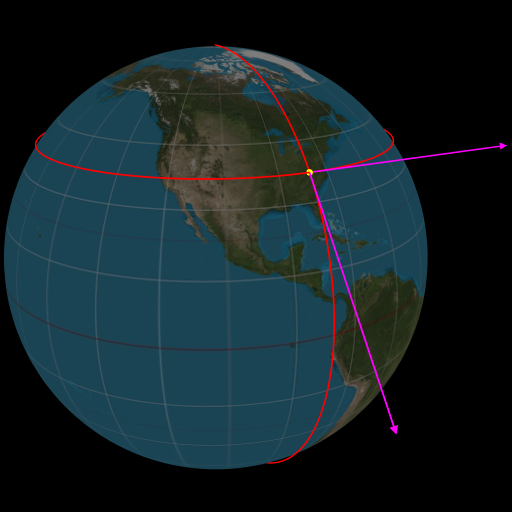
\includegraphics[width=\linewidth]{ex2.png}
    \caption{Exemplo 2 - Perspectiva em 3D}
    \label{img:ex2}
\end{figure}

A figura \ref{img:ex2gt} demonstra o geodesic tracing.
\begin{figure}[!ht]
    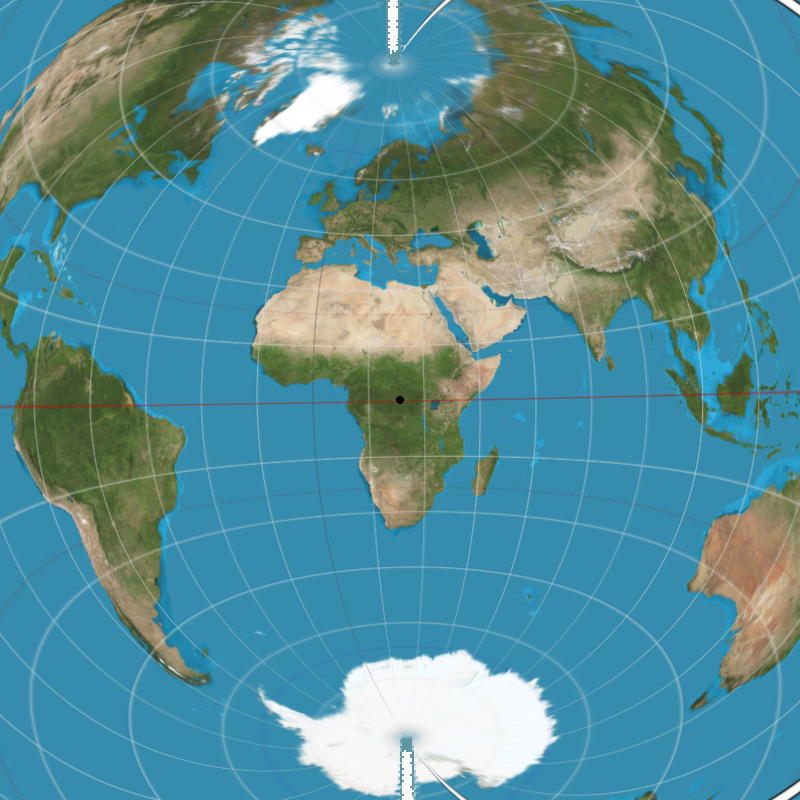
\includegraphics[width=\linewidth]{ex2gt.png}
    \caption{Exemplo 2 - geodesic tracing}
    \label{img:ex2gt}
\end{figure}

\chapter{Curvas e Superfícies}
\label{geomdiff}
O objetivo primário do projeto é visualizar curvas e superfícies.
As curvas são visualizadas apenas em espaço 3D.
As superfícies são visualizadas em espaço 3D e em \textit{geodesic tracing}.

\section{Curvas}
Há duas principais maneiras de se definir uma curva na geometria analítica:
por parametrização e por equação. Esse trabalho apenas consideras curvas paramétricas.

Uma curva pode ser parametrizada por um número real.
Formalmente, uma parametrização é uma função $\gamma : I \rightarrow \mathbb{R}^n$, onde $I$ é um intervalo real.
Nesse trabalho, o intervalo é fechado, e $n=3$.

As curvas são desenhadas através de vários segmentos.
Dada uma partição de $I$ de $k$ pontos,
pode-se aproximar a curva pelos segmentos de extremidade $\gamma(t_{i})$ e $\gamma(t_{i-1})$ para $i<k$,
onde $t_i$ é o i-ésimo ponto da partição. Nesse trabalho, a partição depende apenas de $k$ e é uniforme.

O vetor tangente pode ser calculado com $\gamma'(t)$.

\section{Superfícies}
Assim como as curvas, apenas superfícies parametrizadas serão consideradas nesse trabalho:
$\sigma :  I_1 \times I_2 \rightarrow \mathbb{R}^3$, onde $I_1$ e $I_2$ são intervalos fechados reais.
Além disso, apenas superfícies regulares serão consideradas: a parametrização é suave e
os vetores tangentes são linearmente independentes.

As superfícies são desenhadas através de vários triângulos,
a partir de partições dos intervalos $I_1$ e $I_2$.
Juntas, as partições formam uma grade de retângulos, e cada retângulo pode ser dividido em 2 triângulos.
Esses são os triângulos desenhados.

Os vetores tangentes nas direções coordenadas são as derivadas parciais $\sigma_u(u,v)$ e $\sigma_v(u,v)$, onde os parâmetros são $u$ e $v$.

\subsection{Primeira forma fundamental}
Numa superfície parametrizada regular,
a primeira forma fundamental no ponto paramétrico $(u,v)$ é definida como
\[
    \left[
        \begin{array}{cc}
            \sigma_u \cdot \sigma_u & \sigma_u \cdot \sigma_v \\
            \sigma_v \cdot \sigma_u & \sigma_v \cdot \sigma_v
        \end{array}
    \right]
    = 
    \left[
        \begin{array}{cc}
            E & F \\
            F & G
        \end{array}
    \right]
\]
onde as funções são todas aplicadas no ponto $(u,v)$.

Os vetores $\sigma_u$ e $\sigma_v$ formam uma base do espaço tangente.
O produto escalar de dois vetores tangentes 
$x = x_1 \sigma_u + x_2 \sigma_v$ e $y = y_1 \sigma_u + y_2 \sigma_v$ pode ser calculado da seguinte forma:
\[x\cdot y = (x_1 \sigma_u + x_2 \sigma_v) \cdot (y_1 \sigma_u + y_2 \sigma_v)\]
\[x\cdot y = x_1 y_1 E + x_1 y_2 F + x_2 y_1 F + x_2 y_2 G\]

O produto depende apenas dos coeficientes e da primeira forma fundamental.
Isso significa que distâncias e ângulos podem ser calculados
sem se referir ao espaço ambiente da parametrização, ou seja, de forma intrínseca.

\subsection{Rotação}
Para a aplicação, é necessário rotacionar vetores no espaço tangente.
É possível rotacionar um vetor apenas usando seus componentes e
a primeira forma fundamental.

Seja $w = u\sigma_u+v\sigma_v$ o vetor a ser rotacionado e $\theta$ o ângulo da rotação.
A base $\{\sigma_u, \sigma_v\}$ do espaço tangente pode ser ortogonalizada.
Com uma base ortogonal, a rotação é feita com a matriz de rotação.

A nova base pode ser escrita como:
\begin{align*}
    \sigma'_u &= \frac{\sigma_u}{E}\\
    \sigma'_v &= \frac{\sigma_v-\frac{F\sigma_u}{E}}{R}\\
    R &= \sqrt{EG-F^2}
\end{align*}

Note que os vetores são ortogonais e de mesmo comprimento.
Apesar do comprimento não ser 1, a matriz de rotação funciona corretamente.

Para achar os componentes de $w$ na nova base, basta observar:
$w = u'\sigma'_u+v'\sigma'_v = u'\frac{\sigma_u}{E} + v'\frac{\sigma_v}{R}-v'\frac{\sigma_uF}{RE}$

Então
\begin{align*}
    u' &= uE + vF\\
    v' &= vR
\end{align*}

O vetor rotacionado é
\[w' = \left(u'\text{cos}\theta-v'\text{sin}\theta\right)\sigma'_u + \left(u'\text{sin}\theta+v'\text{cos}\theta\right)\sigma'_v\]
\[w' = \left(u\text{cos}\theta-\frac{uF+vG}{R}\text{sin}\theta\right)\sigma_u+\left(\frac{uE+vF}{R}\text{sin}\theta+v\text{cos}\theta\right)\sigma_v\]

Como esperado, esse vetor só depende da primeira forma fundamental,
dos componentes originais e do ângulo de rotação.

\subsection{Transporte Paralelo}
Seja $\gamma$ uma curva sobre a superfície e $v$ um campo vetorial tangente sobre a curva $\gamma$.
Diz-se que $v$ é paralelo ao longo de $\gamma$ quando $v'$ é ortogonal à superfície
para qualquer ponto de $\gamma$.
Nesse caso, um ser sobre a superfície não observaria mudanças em $v$ ao traçar a curva $\gamma$.
A variação de $v$ se dá ortogonalmente à superfície, logo não seria percebida pelo ser.
Diz-se que o vetor $v$ está sendo transportado paralelamente ao longo de $\gamma$.

Sejam $v$ e $w$ vetores paralelos ao longo de $\gamma$(transportados paralelamente).
Então o produto escalar $v \cdot w$ é constante, pois $(v \cdot w)' = v' \cdot w + v \cdot w' = 0$.
Como o produto escalar pode definir as noções de comprimento e ângulo, vetores transportados
paralelamente à uma curva mantém seus comprimentos e ângulos entre si.

\subsection{Equação geodésica}
Uma curva regular $\gamma$ sobre a superfície é dita geodésica quando
$\gamma'$ é paralelo ao longo de $\gamma$.
Nesse caso, um ser perceberia $\gamma'$(velocidade) como constante, e a curva $\gamma$ pode
ser considerada como reta nesse espaço.

Uma curva $\gamma$ é uma curva geodésica quando satisfaz o sistema \ref{geoeq} \cite{GeomDiff:1}.
\begin{equation}
\label{geoeq}
    \left\{\begin{array}{cc}
        \dfrac{1}{2}\left(E_u(u')^2 + 2F_uu'v' + G_u(v')^2\right) & = \dfrac{d}{dt}(Eu' + Fv') \vspace{6pt}\\
        \dfrac{1}{2}\left(E_v(u')^2 + 2F_vu'v' + G_v(v')^2\right) & = \dfrac{d}{dt}(Fu' + Gv')
    \end{array}\right.
\end{equation}

Esse sistema pode ser reescrito como o sistema \ref{geoeq2}.

\begin{equation}
\label{geoeq2}
        2
        \begin{pmatrix}
            E & F \\
            F & G
        \end{pmatrix}
        \begin{pmatrix}
            u'' \\
            v''
        \end{pmatrix}
        =
        \begin{pmatrix}
            v'^2(G_u-2F_v)-u'^2E_u-2u'v'E_v \\
            u'^2(E_v-2F_u)-v'^2G_v-2u'v'G_u
        \end{pmatrix}
\end{equation}

Como a superfície é regular, $u''$ e $v''$ são únicos, pois a primeira forma
fundamental é invertível.

Note que a aceleração $(u'', v'')$ pode ser obtida em função da posição $(u,v)$
e velocidade $(u', v')$: $(u'', v'') = g(u, v, u', v')$.

Esse é um sistema de equações diferenciais ordinárias de primeira ordem.
Sua solução depende de uma posição e uma velocidade inicial.
Na maioria das superfícies interessantes, esse sistema é muito difícil, ou até impossível,
de resolver analiticamente.

\subsection{Geodesic Tracing}
A visualização do Geodesic Tracing requer uma imagem sobre a superfície.
Para isso, uma cor é associada a cada ponto $(u,v)$ do domínio da parametrização.

O geodesic tracing gera uma imagem a partir de duas informações:
\begin{itemize}
    \item um ponto $(u,v)$ da superície, representando a posição da câmera
    \item dois vetores tangentes $X$ e $Y$ no ponto $(u,v)$.
    Os vetores $X$ e $Y$ são de mesmo comprimento($z$), são ortogonais entre si e
    representam a orientação da câmera.
\end{itemize}

A imagem gerada é um quadrado $[-1, +1] \times [-1, +1]$.
O primeiro eixo corresponde ao vetor $X$, e o segundo ao $Y$.

Cada ponto $(x,y)$ é associado a um ponto $(u_1, v_1)$ da superfície,
e logo a um ponto da imagem original, obtendo-se uma cor.
O ponto $(u_1, v_1)$ é determinado traçando-se uma curva geodésica $\gamma$.
A posição inicial de $\gamma$ é $(u,v)$, e a velocidade inicial é $xX+yY$.
Finalmente, o ponto $(u_1, v_1)$ é definido como $\gamma(1)$.
A distância percorrida, ou comprimento de arco, é o próprio comprimento
da velocidade inicial: $z\sqrt{x^2+y^2}$.

A figura \ref{img:geotracing} ilustra o geodesic tracing.
Os vetores em rosa são os vetores $X$ e $Y$, ancorados na câmera, o ponto amarelo.
O vetor azul é uma combinação linear de $X$ e $Y$, e portanto está no espaço tangente.
O ponto da superfície observado pelo vetor azul é o final da curva vermelha, o ponto azul.
A curva é uma geodésica com velocidade initial igual ao vetor azul, partindo do ponto amarelo.

\begin{figure}[!ht]
    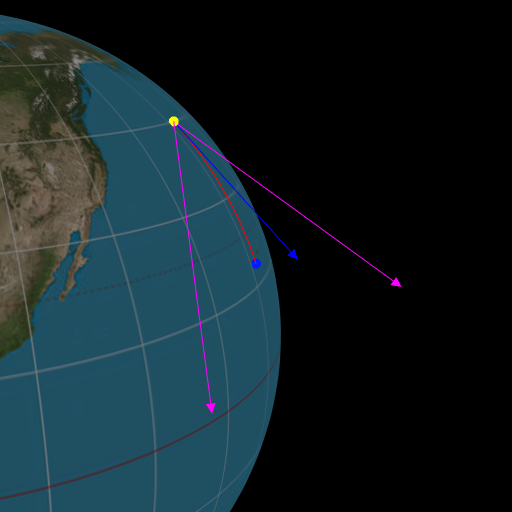
\includegraphics[width=\linewidth]{geotracing.png}
    \caption{Ilustração do geodesic tracing}
    \label{img:geotracing}
\end{figure}

\subsection{Interação}
Para compreender melhor o geodesic tracing,
é necessário alterar as condições e observar as alterações na imagem.

A interação mais simples é a rotação.
Os vetores $X$ e $Y$ são apenas rotacionados por um ângulo $\theta$.
A imagem resultante não se deforma, apenas é rotacionada pelo mesmo ângulo $\theta$.

Outra interação simples é o \textit{zoom}.
Os vetores $X$ e $Y$ são multiplicados por um fator $\alpha > 0$.
Para $\alpha > 1$, a imagem é ampliada, pois as curvas geodésicas são maiores.
Para $\alpha < 1$, a imagem é contraída.

A interação mais interessante é o movimento.
Para se mover na direção $X$, uma geodésica $\gamma$ é traçada na direção $X$.
O novo centro da imagem passa a ser $\gamma(t)$, onde $t$ é o tamanho do passo.
O novo vetor $X$ é a velocidade final($\gamma'(t)$),
que foi transportada paralelamente ao longo
de $\gamma$. O comprimento de $X$ foi preservado.
O novo vetor $Y$ também é transportado paralelamente.
Como visto anteriormente, seu comprimento é preservado e seu ângulo com $X$ também.
Assim, o novo $Y$ é apenas a rotação de $X$ pelo ângulo de $90$ graus.
O comprimento real do passo é $zt$.
De forma similar, a câmera pode se movimentar ao longo de $Y$.

As curvaturas da superfície causam distorções na imagem observada.
Ao se mover, pode-se perceber curvatura pela forma com que a imagem se distorce.
Curvatura gaussiana positiva faz os ``objetos'' expandirem ao se afastar.
Curvatura negativa faz os ``objetos'' contraírem ao se afastar.

%\chapter{Desenvolvimento}

Corresponde ao corpo do trabalho, contendo a exposição ordenada e pormemorizada
do assunto. Constam aqui a revisão de literatura, metodologia adotada, os resultados e
sua discussão. Divide-se em seções e subseções. \cite{Robert2007}


%\chapter{Conclusions}
\label{ch:conclusions}




% -----------------------------------
% ELEMENTOS PÓS-TEXTUAIS
% -----------------------------------
\postextual
% ----------------------------------

%\bibliography{biblio}
\printbibliography

%\glossary

% ----------------------------------------------------------
% Apêndices
% ----------------------------------------------------------

% ---
% Inicia os apêndices
% ---
% \begin{apendicesenv}

% % Imprime uma página indicando o início dos apêndices
% \partapendices

% \end{apendicesenv}
% ---

% ----------------------------------------------------------
% Anexos
% ----------------------------------------------------------

% \begin{anexosenv}

% \partanexos

% \end{anexosenv}

%---------------------------------------------------------------------
% ÍNDICE REMISSIVO
%---------------------------------------------------------------------
\phantompart
\printindex

\end{document}